\documentclass[tikz,border=6pt]{standalone}
\usepackage[T1]{fontenc}
\usepackage{newtxtext,newtxmath}
\usepackage{xcolor}
\usepackage[hidelinks]{hyperref}
\usetikzlibrary{arrows.meta,positioning,calc}
\begin{document}
{\hypersetup{hidelinks}%
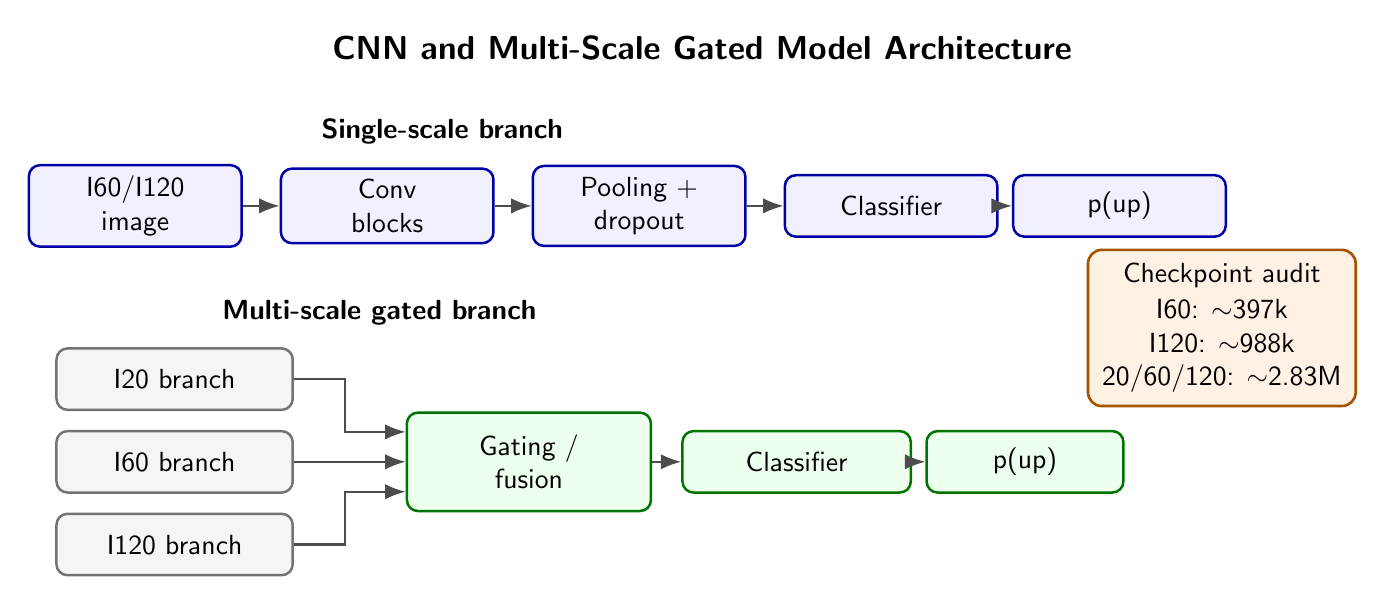
\begin{tikzpicture}[
    font=\sffamily,
    >=Latex,
    basebox/.style={rounded corners=4pt, line width=0.9pt, minimum height=0.78cm, align=center, inner sep=4pt},
    title/.style={font=\sffamily\bfseries\large, align=center},
    subtitle/.style={font=\sffamily\bfseries\normalsize, align=center},
    arrow/.style={-{Latex[length=2.6mm]}, line width=0.75pt, draw=black!70},
    bluebox/.style={basebox, draw=blue!65!black, fill=blue!6, minimum width=2.7cm},
    greenbox/.style={basebox, draw=green!45!black, fill=green!7, minimum width=2.9cm},
    greybox/.style={basebox, draw=black!55, fill=black!4, minimum width=3.0cm},
    auditbox/.style={rounded corners=5pt, draw=orange!65!black, line width=0.95pt, fill=orange!10, align=center, inner sep=5pt}
]
\node[title] at (8.5,0) {CNN and Multi-Scale Gated Model Architecture};
\node[subtitle] at (5.2,-1.05) {Single-scale branch};
\node[bluebox] (s1) at (1.3,-2.0) {I60/I120\\image};
\node[bluebox] (s2) at (4.5,-2.0) {Conv\\blocks};
\node[bluebox] (s3) at (7.7,-2.0) {Pooling +\\dropout};
\node[bluebox] (s4) at (10.9,-2.0) {Classifier};
\node[bluebox] (s5) at (13.8,-2.0) {p(up)};
\draw[arrow] (s1.east) -- (s2.west);
\draw[arrow] (s2.east) -- (s3.west);
\draw[arrow] (s3.east) -- (s4.west);
\draw[arrow] (s4.east) -- (s5.west);
\node[subtitle] at (4.4,-3.35) {Multi-scale gated branch};
\node[greybox] (m20) at (1.8,-4.20) {I20 branch};
\node[greybox] (m60) at (1.8,-5.25) {I60 branch};
\node[greybox] (m120) at (1.8,-6.30) {I120 branch};
\node[greenbox, minimum width=3.1cm, minimum height=1.25cm] (fusion) at (6.3,-5.25) {Gating /\\fusion};
\node[greenbox, minimum width=2.9cm] (clf) at (9.7,-5.25) {Classifier};
\node[greenbox, minimum width=2.5cm] (pup) at (12.6,-5.25) {p(up)};
\draw[arrow] (m20.east) -- ++(0.65,0) |- ($(fusion.west)+(0,0.38)$);
\draw[arrow] (m60.east) -- ($(fusion.west)+(0,0)$);
\draw[arrow] (m120.east) -- ++(0.65,0) |- ($(fusion.west)+(0,-0.38)$);
\draw[arrow] (fusion.east) -- (clf.west);
\draw[arrow] (clf.east) -- (pup.west);
\node[auditbox, minimum width=3.4cm, minimum height=1.65cm] (audit) at (15.1,-3.55) {Checkpoint audit\\[1pt]I60: $\sim$397k\\I120: $\sim$988k\\20/60/120: $\sim$2.83M};
\end{tikzpicture}%
}
\end{document}
